\chapter{Background Theory}
\label{chapter:Background}
In this chapter, the theoretical background for the implementation of the \textit{CAD-integrated Topology Optimization} tool is presented. The chapter is divided into four sections: \emph{\nameref{sec:CADbackg}} (\autoref{sec:CADbackg}), \emph{\nameref{sec:TopOpt}} (\autoref{sec:TopOpt}), \emph{\nameref{sec:surfaceBackg}} (\autoref{sec:surfaceBackg}), and \emph{\nameref{sec:NURBS}} (\autoref{sec:NURBS}).
\todourgent[inline] {anyone: update Background description with Least-squares section, and scan rest of document for inconsistencies re: this section nod added}
%overview over CAD
\section{CAD overview}
\label{sec:CADbackg}
\todointern[inline]{Explain voxelization}
%interaction with it, programs, geometry represenations, datastructures, formats etc., maybe even history if we're overkill
\Acf{CAD} refers to the process of designing a product using a computer system. Before \ac{CAD} applications were used, products were designed using a sketch board. It was a challenge to incorporate changes in the construction drafts as well as to keep documentations up to date; hence, it was no surprise that \ac{CAD} systems spread rapidly across all design development branches. \Ac{CAD} is now of irreplaceable use in architecture, mechanical, electrical and civil engineering.

Depending on the discipline, different requirements are set on the virtual model. One may imagine that in a civil engineering model of a building a 2D floor plan is often sufficient; however, in the design of a mechanical motor a 3D model is always necessary. Given these circumstances, various \ac{CAD} software bundles evolved in the different disciplines with completely different modelling approaches. Besides the geometry representation additional parameters, such as material properties or manufacturing information, are stored. In order to move between different data structures standardized exchange interfaces are commonly used. 

This section presents the relevant geometrical and computational aspects of \ac{CAD} for the project; for a more thorough introduction we refer to \cite{sarcarCAD}.

\subsection{Geometry representations}
\todointern[inline]{Saumitra: Repetitive use of names, review}
In general, two different ways of describing a geometry are used in \ac{CAD} systems: a \acf{CSG} or a \acf{BREP}. Other approaches, such as a complete voxelised geometry are not common due to extensive memory consumption.
\subsubsection{\Acl{CSG}}
\begin{figure}
\centering
\includegraphics[width=0.5\textwidth]{Pictures/Csg_tree.png}
\caption{\ac{CSG} object tree. The picture shows the construction of a complex object from a cube, a sphere, and a set of cylinders. Figure taken from \cite{WikipediaCSG}.}
\label{fig:csg_tree}
\end{figure}
One way of representing a geometry in \ac{CAD} is the approach of \ac{CSG}. The basic idea is to start from a set of primitives, e.g. spheres, cylinders and/or cubes. Basic Boolean operations link these primitives towards a complex geometry, as illustrated in \autoref{fig:csg_tree}.

Key advantages of this format is the precise representation using very little storage memory. However, not all desired forms can be represented by \ac{CSG} and hence, a second type of geometry description is needed. 
\subsubsection{\Acl{BREP}}
A different kind of modelling approach is the \ac{BREP}. Instead of storing the geometry information as geometrical objects, \ac{BREP} formats only save the boundary surface of the body. The interior is assumed to be uniformly filled. Especially in complex geometries, this approach simplifies the model to such an extent, that the amount of data becomes much easier to handle. Surfaces can then be for example stored as a set of triangles (as in \ac{STL} files, see \autoref{subsub:STL} below) or in \ac{NURBS} \acsp{patch} (see \autoref{sec:NURBS}).
Furthermore, holes in the body are made possible by saving the surface normal of the respective boundary. 

By the boundary representation arbitrary geometries can be created. While the data sizes are commonly larger than in \ac{CSG} representation, \ac{BREP} files are usually easier to work with. One also has to keep in mind, that non-physical geometries can result from \ac{BREP} formats through a not closed surface.
\subsection{Data exchange interfaces}
\ac{CAD} software programs usually use their own data formats; in order to exchange models standardized interface formats have been developed. Geometric models are compressed to certain geometry descriptions; transferring additional information, such as material properties or manufacturing information, is in general a difficult task and in some exchange file formats even prohibited. A few common exchange file types are described below, as also compared in \cite{STL}.
\subsubsection{\acs{STL} file format} \label{subsub:STL}
The \acf{STL} file format describes the model only by its boundary and is thus a \ac{BREP} format. The idea behind its files is simple. The geometric model is discretized into a cloud of points, where sets of three vertices form a triangle; hence, a connected surface of triangles emerges which describes the geometry. The procedure is shown in \autoref{fig:STL} for a two dimensional circle.  
\begin{figure}
\centering
   \scalebox{0.4}{\includegraphics{Pictures/STL.pdf}}\\
   \caption{\ac{STL} discretization for a circle, self-made in MATLAB \cite{MATLAB}. Note that the circle cannot be exactly represented by the vertices and edges.}
   \label{fig:STL}
\end{figure}
The aforementioned triangles boil down to lines in two dimensions. The advantages and disadvantages of this approach become clear: It can be applied to an arbitrary geometry, but accuracy causes difficulties. In order to transfer high precision geometries many vertices are necessary, resulting in big files. Still, as is illustrated in the figure, a perfect circle can never be represented. 

ASCII \ac{STL} files begin with a name and the data on the triangles is constructed as follows: 
\begin{itemize}
\item a facet normal pointing outward
\item a sequence of vertex coordinates
\end{itemize}
As this is the only information provided, no additional data such as material properties are transferred through \ac{STL} files, reducing file size but also range of usage.
\subsubsection{\acs{STEP} and \acs{IGES} file formats}
To overcome issues of insufficient precision also more elaborate exchange formats exist; these save e.g. a circle as a parameter where no discretization step is involved. Also, the possibility of passing additional parameter information (e.g. density, manufacturing information) is required by certain users. Popular file types that offer these two functionalities are \acf{STEP} and \acf{IGES} files. 

The \ac{STEP} file format is a newly developed \ac{CAD} data exchange standard and documented in the ISO 10303 norm. On the contrary to \ac{STL} files it uses a combination of \ac{CSG} and \ac{BREP} to store the geometry. Additional information (e.g. density, color) are passed through attribute sets that are stored besides geometry instances (e.g. a circle). A key disadvantage, however, is that \ac{STEP} files carry much redundant information \cite{STL}.


The \acl{IGES} is an American National Standard since 1981 to exchange graphics information. Similar to the \ac{STEP} format it uses a combination of \ac{CSG} and \ac{BREP} for the geometry representation. Instead of storing a set of manufacturing information as done in the \ac{STEP} file, the \ac{IGES} is build only to exchange graphics information. For example, the \ac{STEP} file transfers a physical density information; in the \ac{IGES} format the only additional parameter stored on a node is the coloring information. Consequentially, \ac{IGES} file sizes are significantly smaller compared to the \ac{STEP} file format \cite{STL}.

The \ac{IGES} file format contains five different sections: a \emph{Start}, \emph{Global}, \emph{Directory Entry}, \emph{Parameter Data} and \emph{Terminate} section. The \emph{Start} and \emph{Global} section are used for naming and part information. In the \emph{Directory Entry} section additional information like the node color is saved. The \emph{Parameter Data} section is used for storing the coordinate points; the \emph{Terminate} section signals the end of the file \cite{sarcarCAD}.


%how the algorithms work, maybe what it can be used for
\subsection{Definition and motivation}
Topology Optimization describes the process of finding the optimal distribution of a limited amount of material for a given area or volume based on a predefined constraint/minimization problem. Possible optimization goals are for example:
\begin{itemize}
\item \textbf{Minimum compliance} which seeks to find the optimal distribution of material that returns the stiffest possible structure. The structure is thereby subjected to loads (forces) and supports (boundary conditions). By maximizing the stiffness, we minimize the compliance.
\item \textbf{Heat conduction} tries to optimize the domain of a conductive material with respect to conductivity for the purpose of heat transfer. This maximization problem is the same as minimizing the temperature gradient over the domain-- a poor conductor will create a large gradient.
\item \textbf{Mechanism synthesis}' objective is to obtain a device that can convert an input displacement in one location to an output displacement in another location. Topology Optimization hereby seeks the optimal design which maximizes the output force for a given input or, respectively, minimizes the input force for a given output.
\end{itemize}


As one can imagine by this short list of optimization goals, Topology Optimization has a wide field of possible applications. Hence, it has become a well established technology used by engineers in the fields of aeronautics, civil, materials, mechanical and structural optimization. Furthermore, the rising significance of 3D-printers in industry, the realisation of computed optimized designs is now much easier.

\subsection{Theory}
%Maybe a little theory here about how topology optimization actually works

\subsection{ToPy}
ToPy \cite{ToPy} is a python library/program, written by William Hunter and documented in \cite{Hunter2009}. It is based on the 99-line Matlab code by Sigmund's for minimum compliance. The program can optimize the three above named problem types, minimum compliance, heat conduction and mechanism synthesis-- in 2D as well as 3D. It uses available open source python software, as for example Pysparse and Numpy, leading to improved speed, porta- and scalability. The whole program is steered by an input file which-- with the help of the documentation-- is straightforward to use and easy to adapt. 

\subsection{Implementation}
In terms of our implementation, we use ToPy as a blackbox topology optimizer. This means, we launch the program with an input file based on our scenario, let ToPy run and proceed by working with the output of ToPy. The intention is to touch the solver itself as less as possible to be able to just plug in different solvers later on. Implementation-wise that means, that we wrote a program which takes as input a voxelized CAD design in, for example, stl-format and outputs a tpd-file which can be used by ToPy. Results of the process can be seen in figure \ref{fig: topyStar}. Here, a star was given as input from a stl-file. We fixed the voxels in the corners of the structure, while we set a load in the middle, pointing into the structure. As can be seen, the optimization process "cuts" away unnecessary material in-between the corners and even in the middle of the material and returns stiff structure for a minimal amount of material. (maybe a bit wishy washy here)
\begin{figure}
\centering
\begin{subfigure}{
  \includegraphics[width=.2\linewidth]{Pictures/TopOp/Star_Optimized0_Trans.png}}
\end{subfigure}%
\begin{subfigure}{
  \includegraphics[width=.2\linewidth]{Pictures/TopOp/Star_Optimized2_Trans.png}}
\end{subfigure}
\begin{subfigure}{
  \includegraphics[width=.2\linewidth]{Pictures/TopOp/Star_Optimized4_Trans.png}}
\end{subfigure}
\begin{subfigure}{
  \includegraphics[width=.2\linewidth]{Pictures/TopOp/Star_Optimized5_Trans.png}}
\end{subfigure}
\caption{Topology Optimization with minimum compliance of a star structure, given by an stl-file. The fixtures were applied in the corners of the star, while a load was set in the middle.}
\label{fig: topyStar}
\end{figure}


%section moved to implementation
%\section{From CAD to Voxels}
%%\subsection{Motivation}
%The goal of good design is to find the right balance between a set of parameters, which usually include efficiency, weight and aesthetics. For a long time, this process had been an ardous loop of minute modifications to the product, oscillating between the engineer and the designer. However, with the advent of Topology optimization (see \autoref{sec:TopOpt}) and additive manufacturing, it has been shrunk drastically to an efficient, compact task. In the previous section, we summarized the different ways of representing a design object digitally. On specifying the appropriate loads as boundary conditions on this object, one can choose their favourite topology optimization tool to compute the optimal dimensions and form.


The main hurdle with most state-of-the-art open source topology optimization tools is their input format, where many of them require input to be specified as a 3-dimensional voxel grid. Presence (or absence) of material in these voxels is defined by a boolean variable, and boundary conditions are imposed on the appropriate locations. %This section describes how we overcame this hurdle of converting CAD representations to voxelized input.



% section on Surface Extraction methods

\subsubsection{Dual Contouring}

\begin{frame}
	\frametitle{From Voxel to Mesh Geometry}
	Task:
	\begin{itemize}
	\item Extract isosurface from voxel information
	\item Algorithms: Marching Cubes, Dual Contouring, Extended Models
	\end{itemize}
	Steps: 
	\begin{enumerate}
		\item Locate the position of the vertex inside each cube which has at least one sign changing
		edge
		\item Join the vertices associated with four cubes sharing a common edge to form a quadrilateral face (quad)
	\end{enumerate}
	\begin{minipage}{0.49\textwidth}
	\only<1>{
	\begin{figure}	
	\centering
	\includegraphics[width=.35\textwidth]{Pictures/DC/MC1.png}\caption{Marching cube}
	\end{figure}}
	\only<2>{
		\begin{figure}	
		\centering
		\includegraphics[width=.35\textwidth]{Pictures/DC/MC2.png}\caption{Marching cube}
		\end{figure}}
	\only<3>{
		\begin{figure}	
		\centering
		\includegraphics[width=.35\textwidth]{Pictures/DC/MC3.png}\caption{Marching cube}
		\end{figure}}
			\only<4>{
				\begin{figure}	
				\centering
				\includegraphics[width=.35\textwidth]{Pictures/DC/MC4.png}\caption{Marching cube}
	\end{figure}}
	\end{minipage}
	\begin{minipage}{0.49\textwidth}
	\only<1>{
	\begin{figure}	
	\centering
	\includegraphics[width=.35\textwidth]{Pictures/DC/MC1.png}\caption{Dual Contouring}
	\end{figure}}
	\only<2>{
		\begin{figure}	
		\centering
		\includegraphics[width=.35\textwidth]{Pictures/DC/MC2.png}\caption{Dual Contouring}
		\end{figure}}
	\only<3>{
		\begin{figure}	
		\centering
		\includegraphics[width=.35\textwidth]{Pictures/DC/DC3.png}\caption{Dual Contouring}
		\end{figure}}
			\only<4>{
				\begin{figure}	
				\centering
				\includegraphics[width=.35\textwidth]{Pictures/DC/DC4.png}\caption{Dual Contouring}
	\end{figure}}
	
	\end{minipage}
%	\caption{Comparision of MC and DC for identical datasets. The vertices are created on the edges of the cubes for MC  and inside the cubes for DC. Please note that the sharp feature in the top right cube can only be reconstructed by DC. Figure from %\cite{FromVoxelsToPolygons}.
\end{frame}


\begin{frame}
	\frametitle{Two-grid Dual Contouring}
	\begin{overlayarea}{\textwidth}{0.9 \textheight}
	\begin{minipage}{0.45\textwidth}
	\begin{block}{\centering Coarse grid}
	\vspace{-0.5cm}
	\begin{figure}
	\includegraphics[scale=0.35]{Pictures/DC/DC_1_Coarse.pdf}
	\end{figure}
	\begin{itemize}
	\item Coarse quads used in \textcolor{red}{parametrization}
	\end{itemize}
	\end{block}
	\end{minipage}
	\hfill%
	\begin{minipage}{0.45\textwidth}
	\begin{block}{\centering Fine grid}
	\vspace{-0.5cm}
	\begin{figure}
	\includegraphics[scale=0.35]{Pictures/DC/DC_1_Fine.pdf}
	\end{figure}
	\begin{itemize}
	\item Fine vertices used for \textcolor{red}{projection}
	\end{itemize}
	\end{block}
	\end{minipage}
	\end{overlayarea}
\end{frame}

%\subsection{B--Spline}

\subsection{Projection and Parametrization}
\begin{frame}{Projection and Parametrization}
%\framesubtitle{Least square fitting}
\begin{overlayarea}{\textwidth}{.9 \textheight}
%\begin{minipage}{0.45\textwidth}
\begin{enumerate}
\visible<1->{\item Use coarse quad from Dual Contouring}
\visible<2->{\item Project grid points from fine grid onto plane}
\visible<3->{\item Find corresponding parameters for B-Spline surface $\left[u,v\right] \in \left[0,1\right]^2$}
\visible<4->{\alert<4->{\item[$\Rightarrow$] Peter's scheme}}
\end{enumerate}
%\end{overlayarea}
%\begin{overlayarea}{\textwidth}{.85 \textheight}
%\end{minipage}
\vspace{-0.5cm}
%\begin{columns}
%\column{.35\textwidth}
%\begin{overlayarea}{\textwidth}{\textheight}
\begin{figure}
\visible<1->{
\tdplotsetmaincoords{60}{110}
\begin{tikzpicture}[scale = 1.5,tdplot_main_coords]
\coordinate (O) at (-1,-1,0);
\coordinate[dot] (A) at (0,0,0);
\coordinate[dot] (B) at (1,0,0);
\coordinate[dot] (C) at (1.2,1.5,0);
\coordinate[dot] (D) at (0,1,0);
\visible<3->{
\coordinate[dot] (E) at (1.4,2.0,-0.5);
\coordinate[dot] (F) at (0,1.7,-0.8);
\draw[thick] (D) -- (F) -- (E) -- (C);}

\coordinate (P1) at (.5,.4,1);
\coordinate (P2) at (1,1,1);
\coordinate (P3) at (0.2,0.2,2);
\coordinate (P4) at (0.1,1.3,1);


\coordinate (Q1) at (.5,.4,0);
\coordinate (Q2) at (1,1,0);
\coordinate (Q3) at (0.2,0.2,0);
\coordinate (Q4) at (0.1,0.9,0);



\draw[thick,->] (O) -- ($(O)+(.5,0,0)$) node[anchor=north east]{$x$};
\draw[thick,->] (O) -- ($(O)+(0,.5,0)$) node[anchor=north west]{$y$};
\draw[thick,->] (O) -- ($(O)+(0,0,.5)$) node[anchor=south]{$z$};

\draw[thick] (A) -- (B) -- (C) -- (D) -- (A);

\visible<2-4>{
\draw (P1) node[thick,cross,red,label = {$P_1$}] {};
\draw[red,dashed] (P1) -- (Q1);
\draw (Q1) node[thick,cross,red] {};
\draw (P2) node[thick,cross,red,label = {$P_2$}] {};
\draw[red,dashed] (P2) -- (Q2);
\draw (Q2) node[thick,cross,red] {};
\draw (P3) node[thick,cross,red,label = {$P_3$}] {};
\draw[red,dashed] (P3) -- (Q3);
\draw (Q3) node[thick,cross,red] {};
}
\visible<3->{
\draw (P4) node[thick,cross,red,label = {$P_4$}] {};
\draw[red,dashed] (P4) -- (Q4);
\draw (Q4) node[thick,cross,red] {};

}
\draw (A) node[label = left:{$A$}]{};
\draw (B) node[label = left:{$B$}]{};
\draw (C) node[label = right:{$C$}]{};
\draw (D) node[label = right:{$D$}]{};
\visible<3->{
\draw (E) node[label = right:{$E$}]{};
\draw (F) node[label = right:{$F$}]{};}
\visible<3->{
\coordinate[dot] (A2) at (0,0,1);
\coordinate[dot] (B2) at (1,0,1);
\coordinate[dot] (D2) at (0.,1.5,0.9);
\coordinate[dot] (C2) at (1,1.9,1);
\draw [dashed] (A2)--(D2) --(C2) -- (B2) -- (A2);
%\draw (C2) node[label = right:{$C'$}]{};
%\draw (D2) node[label = right:{$D'$}]{};
%\draw (A2) node[label = right:{$A'$}]{};
%\draw (B2) node[label = right:{$B'$}]{};
}
\end{tikzpicture}
}
\end{figure}
%\end{overlayarea}

%\column{.5\textwidth}
%\begin{overlayarea}{\textwidth}{\textheight}
%\only<3->{
%\begin{block}{Problem:}
%\begin{itemize}
%\item Fit B-Spline surface, that is C0 and C1 continuous on the borders
%\end{itemize}
%\end{block}
%
%\begin{block}{Solution:}
%\begin{enumerate}
%\item Method: Peter's scheme
%\item Solve (coupled) global system of equations
%\end{enumerate}
%\end{block}
%
%}
%\end{overlayarea}
%\end{columns}
\end{overlayarea}
\end{frame}

%\begin{frame}
%
%	\frametitle{Projection and Parametrization}
%	
%	\begin{itemize}
%	\item Points from finer grid are projected to quads of the coarser grid 
%	\item Parameters \textit{u} and \textit{v} are found for each quad
%	\item This information is needed for the algorithms in the last part of the pipeline
%	\end{itemize}
%	\begin{figure}
%	\includegraphics[scale=0.35]{Pictures/DC/DC_2.pdf}
%	\end{figure}
%	
%\end{frame}







% is this needed??? SOME REMARK ABOUT THIS WILL BE USED IN THIS 
% %%%%%% THIS PART WILL BE INCLUDED IN THE NEXT M. in case this approach is needed.

\subsection{Voxel Data to NURBS}
\todo[inline]{what about this part? talk to Juan Carlos!}
There are two possible roads to go from the voxel data to the CAD representation (in our case NURBS based representation).
\subsubsection{Quad Contouring}
This approach uses the Dual Contouring algorithm as first step in order to obtain a quad mesh representation from the voxel data. The first challenge is to implement the algorithm with the ideas presented in \cite{Hermite2002} correctly. The original Marching Cubes algorithm is implemented in VTK but the source code is not public. Once this first step is done, the quads will be chosen for the NURBS parametrization. A second step considers multiple smaller quads which have to be combined into one larger patch. This is another challenge, since the remeshing of quad meshes is not as straightforward as with the triangles. Different approaches have been taken in order to achieve this coarsening. In \cite{Puppo2010} an incremental and greedy approach, which is based on local operations only, is presented. It depicts an iterative process which performs local optimizing, coarsening and smoothing operations. Other approaches, like the one presented in \cite{Dong2005} uses smooth harmonic scalar fields to simplify the mesh.

2= “Practical quad mesh simplification”
3= “Harmonic Functions for Quadrilateral Remeshing of Arbitrary Manifolds”


\subsubsection{Multiresolution Analysis of Arbitrary Meshes}
With \textit{Multiresolution Analysis of Arbitrary Meshes} approach there is no need to apply a Dual Contouring algorithm, since it takes as beginning data the triangles from the Marching Cubes. The main concepts are shown in the paper \cite{eck1996automatic}. It mainly takes a series of intermediate steps which permits a parametrization of data. It includes a partitioning scheme based on the ideas of the Voronoi Diagrams \todo{reference} Delaunay triangulations \todo{reference}.Large patches or quads are obtained with this method. 

4=reference to MAAM, a.k.a Benni's favorite paper!

\subsubsection{implementation part!}
Both approaches have not been implemented in open source documentation, therefore there is a need to implement it from scratch. Up to now, the second approach has been chosen.

% section on the whole fitting process from a reconstructed surface to NURBS
\section{Fitting \acs{NURBS} to data}
\label{sec:NURBS}

\todo[inline]{expand this! and a better name}
In this section we will discuss:
\begin{itemize}
\item Parametrized curves and surfaces such as Bezier and NURBS surfaces
\item Peter's scheme, a scheme for generating tangent plane continous ($G^1$) surfaces from an unstructured mesh of polygonal faces as first described in...[ref]
\item Possibly how to fit this surface to parametrized datapoints using least squares. That could be impl.
\end{itemize}

\subsection{Parametric Curves}
\label{subsec:paracurves}
To define NURBS from a mathematical standpoint, we first define so-called \emph{\Bez curves} and use them later for the definition of NURBS. 
\subsubsection{\Bez Curves}
\label{subsub:bezcurvsurf}
A \Bez curve is a \textit{parametric} curve, which is often used for producing a smooth approximation of a given set of data points.
 
An analytical expression for the \Bez curve parametrized by the variable $u$ is given by:
\begin{equation}
\label{eq:beziercurve}
\vec{B}(u)=\sum\limits_{i=0}^n b_i^n(u) \vec{p}_i
\end{equation}
where $\vec{p}_i$ is the $i^{\text{th}}$ control point, $i\in0,1, \dots ,n$ ($n+1$ control points in total), and
\begin{equation*}
b_i^n(u)=\binom{n}{i}(1-u)^{(n-i)}u^i
\end{equation*}
with $\binom{n}{i}$ being a binomial coefficient, is the $i^{\text{th}}$ \emph{Bernstein polynomial} (see \cite{lorentz2012bernstein}) of degree $n$.

In addition to the expression with Bernstein polynomials, one can use a recursion formula (so-called \emph{de Casteljau Algorithm}) for the construction of the \Bez curve, which we will not cover here. 

Analogous to \Bez curves, one can also define a \textit{\Bez surface}. One way of doing this is by extending the set of control points indexed in one dimension, to a two-dimensional mesh of $n\times m$ control points $\vec{p}_{i,j}$. Likewise, we extend the Bernstein polynomial basis to $2$D by taking its tensor product with itself. The resulting \textit{tensor product \Bez surface} is then given by the analytical expression
\begin{equation}
\label{eq:bezsurface}
\vec{S}(u,v)=\sum\limits_{i=0}^n \sum\limits_{j=0}^m b_i^n(u) b_j^m(v) \vec{p}_{i,j}
\end{equation}

\subsubsection{B-Splines and NURBS}
Extending the idea described in previous section, one could use \emph{B-spline basis functions} (see below) instead of the Bernstein polynomial basis.

Unlike \Bez curves, the parameter domain for B-splines is subdivided by so-called \textit{knots}. For the one-dimensional parameter domain $[u_{0}, u_{m}]$, the \textit{knot vector} will be given by $u_{0} \leq u_{1} \leq ... \leq u_{m}$. In most cases $u_{0} = 0, u_{m} = 1$ is chosen, so that we get a unit interval for our parameter values. For the case of NURBS, the knots $u_{0},..., u_{m}$ need not be equidistant -- hence the "NU" (for Non-Uniform) in the name "NURBS".

Given a knot vector $[u_{0}, u_{m}]$ and a degree of B-spline $p$, the $i$-th B-spline basis function is then defined recursively as follows:
\begin{equation}
N_{i,0}(u) =  \begin{cases} 1, & \mbox{if } u_{i} \leq u < u_{i+1} \\ 0, & \mbox{otherwise } \end{cases}
\end{equation} 
\begin{equation}
N_{i}^p(u) = \frac{u - u_{i}}{u_{i+p} - u_{i}}N_{i}^{p-1}(u)  + \frac{u_{i+p+1}-u}{u_{i+p+1} - u_{i+1}}N_{i+1}^{p-1}(u)
\end{equation}
For $p=0$ the basis fucntions are simply step functions, and for $p=1$ we end up with so-called "hat" functions. Quadratic basis functions ($p=2$) look more complicated (\autoref{fig:bsplineBases}).
\begin{figure}
\centering
\begin{subfigure}[b]{.3\linewidth}
  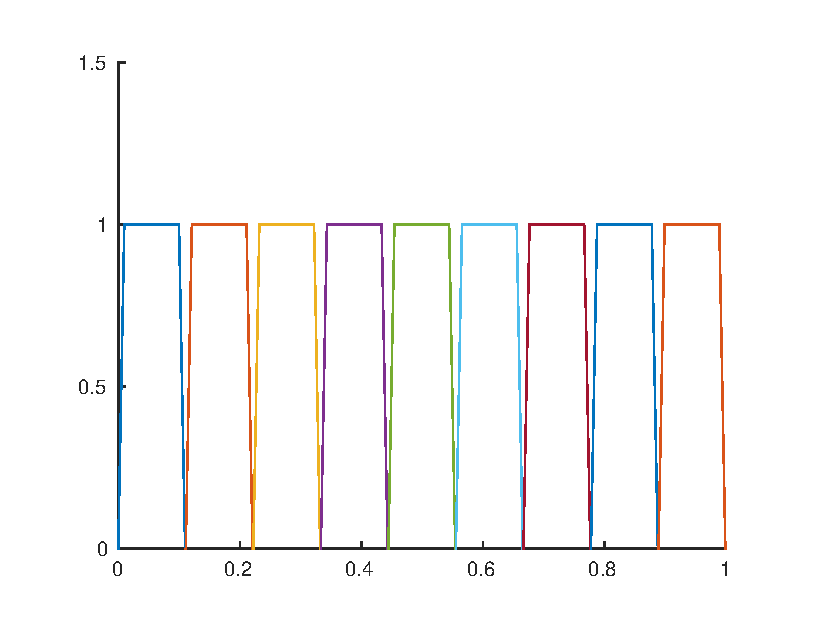
\includegraphics[width=\linewidth]{Pictures/basisconstant}
  \subcaption{B-spline basis for $p=0$}
  \label{fig:bspline_basis_constant}
\end{subfigure}%
\begin{subfigure}[b]{.3\linewidth}
  \includegraphics[width=\linewidth]{Pictures/basislinear}
  \subcaption{B-spline basis for $p=1$}
  \label{fig:bspline_basis_linear}
\end{subfigure}
\begin{subfigure}[b]{.3\linewidth}
  \includegraphics[width=\linewidth]{Pictures/basisquadratic}
  \subcaption{B-spline basis for $p=2$}
  \label{fig:lognorm_quadratic}
\end{subfigure}
\caption{B-spline basis functions, of degree $p=0$ (left), $p=1$ (middle) and $p=2$ (right).}
\label{fig:bsplineBases}
\end{figure}


By giving each of these basis functions a weight $\omega_i$ and normalizing them at each point by dividing by the total sum, we get the rational basis functions. Writing them out explicitly, in terms of B-spline basis functions $N_{i,p}$, the $n^{\text{th}}$-degree NURBS surface with $k$ control points $P_i$ is finally given by:
\begin{equation}
\label{eq:nurbscurve}
\vec{C}(u) = \frac{\sum_{i=1}^{k}N_i^n\left(u\right)\omega_{i}\vec{p}_{i}}{\sum_{i=1}^{k}N_i^n\omega_{i}}.
\end{equation}

B-splines have the following properties, which are useful for our problem:
\begin{itemize}
\item Degree $n$ and number of control points $\vec{P}_{i\cdots m}$ are independent.
\item B-Splines only change locally (depending on the degree $n$) when a control point is changed.
\end{itemize}

Analogous to the tensor product \Bez curve surfaces (see \autoref{eq:bezsurface}), one can define tensor product B-spline or NURBS surfaces:
\begin{equation}
\label{eq:nurbssurface}
\vec{S_\text{NURBS}}(u,v)=\frac{\sum\limits_{i=0}^n \sum\limits_{j=0}^m N_{i}^n(u) N_{j}^m(v) \omega_{i,j}\vec{p}_{i,j}}{\sum\limits_{i=0}^n \sum\limits_{j=0}^m N_{i}^n(u) N_{j}^m(v) \omega_{i,j}},
\end{equation}
where the case with all $\omega_{i,j} = 1$ corresponds to a B-Spline surface; respectively a NURBS surface if any $\omega_{i,j} \neq 1 $. With varying degrees and number of control points, these can be made to fit a variety of shapes. However, as the parameters $u$ and $v$ define a square in their two-dimensional parameter domain, there is a limit to what topologies may be realized with just one such NURBS surface. For example, an open cylinder could be constructed by one such surface where one of the sides meets its own beginning, whereas something with multiple holes - like a double torus, or a non-flat 8-shaped surface, would be impossible. Therefore, when using NURBS, surfaces are most often modelled using a network of connected patches. \todointern{maybe should include an example picture here} For more information about NURBS, see \cite{farin1999nurbs}.

\subsection{Peter's Scheme}
\todo[inline]{insert stuff here}
In this section we will cover the following, reffering to paper[]:
\begin{itemize}
\item How we go from polygonal faces to a set of mesh control points. "patch points", specifying that we're talking about quads, and that we then get 16
\item That for each of these 16 points, we will make a small Bezier patch
\item That if we define the Bezier control points of these patches in a special way, as described in appendix XYZ \todo{TODO: create this appendix, or change this to refer to paper for coefficients}, we get a surface that is $G^1$ continous
\item Maybe describe that we then need for every one of these Bezier patches the locations of the neighbours
\item That the location of a point on the surface defined by parameters $\vec{s} = (u,v)$ depends on the Bezier control points, whose linear dependence on the "patch points" give us coefficients on these "patch points" of the location described by the parameters, as can be seen in \autoref{fig:PetersPoints}
\item Possibly that this can used to fit the location of these "patch points" to a set of datapoints by minimusing a least-squares error 
\end{itemize}
\begin{figure}

\missingfigure{Graphical descirption of all those different points in peter's scheme}
\label{fig:PetersPoints}
\caption{The points in Peter's scheme. As clearly seen in the figure above, this scheme is self-explanatory.}
\end{figure}

\subsection{Fitting problem}
\todo[inline]{is this really nurbs? well maybe. PRobably stuff the Peter's fitting in here and remove some other parts}
In order to represent a given line or surface by Bezier curves or surfaces respectively, just as with NURBS, one has to solve a fitting problem. The goal of it is to fit in a parametric curve to the set of given data points. In the case of interest, the given set of points is a mesh, obtained from surface contouring.
\subsubsection{Fitting problem: Bezier curve}
First we want to find a Bezier-curve $\vec{B}_n\left(u\right)$ of degree $n$ which is approximating a given spline $\vec{s}_m\left(u\right)$ defined by $m$ points in a optimal way. For this purpose we want to minimize the L2-error. This leads to the minimization problem
\begin{equation}
\text{find\ } \underset{\vec{B}_n\in \mathbb{B}_n}{\min} \Ltwonorm{\vec{B}_n-\vec{s}_m}.
\end{equation}
Minimizing the L2-norm is equal to minimizing the functional:
\begin{equation}
F(\vec{B}_n)=\int\limits_{u=0}^{u=1} \left(\vec{B}_n-\vec{s}_m\right)^2\du
\end{equation}
Using the variational principle we get the the system of linear equations
\begin{equation}
A a = b
\end{equation}
where $A$ is the matrix of pair-wise scalar products of basis functions (Bernstein polynomials), $b$ is the vector of scalar products of the given spline $s_{m}$ and basis functions and $a$ is a required vector of coefficients for Bezier curve representation.

\subsubsection{Fitting problem (least squares): NURBS}
\todo[inline]{why (least squares) here and not above? is this consistent?}
Although the approach used above showed good results, it appears to be very computationally intensive. Analogically, one could reduce the original problem to a \emph{regression problem}, which allows us to reduce computational costs. Also, to improve the locality of our solution, from now on we are going to use NURBS basis functions with weights $\omega_{j} = 1$ instead of Bezier curves. For this purpose, we adopted an algorithm, provided in \cite{becker2011advanced}:

Let $X^{0}$ be the $n \times 2$ matrix of the given set of points, $N^{p}$ the basis functions of degree $p$ ($n \times (n+p)$ matrix, where $n$ is the number of points), and $P^{0}$ the control points ($(n+p) \times 2$ matrix).

The original problem can be written as:
\begin{equation}
X_{i}^{0} = \sum\limits_{j=1}^{n+p} P_{j}^{0} N_{i,j}^{p}, \quad i \in \{1,..,n\}
\end{equation}
Or, in short:
\begin{equation}
X^{0} = N^{p} P^{0}
\end{equation}
The above system needs to be solved for the unknown $P^{0}$. This can be done numerically, for example through singular value decomposition. 
%part of implementation

\subsubsection{Fitting Problem: Peter's Scheme}
\todo[inline]{insert stuff here, what's described in peter's scheme, will see where it fits}

%fitting of surfaces and curves
\section{Least-squares fitting of parametrized surfaces}
\tododone[inline]{Erik: define section}
In order to make a surface adhere as closely as possible to our desired form, some fitting is usually required. This typically involves varying some parameters in order to minimize some error. As minimizing the error squared of a function -- for example distance between a calculated point and its desired location -- is an important building block in many practical applications, extensive literature can be found regarding this, especially when the function depends linearly on its input. The field that treats this topic is called \emph{linear least-squares fitting}, and in this section, some selected subtopics relevant to the fitting of \acs{NURBS} is treated.

%\begin{itemize}
%\item Possibly that this can used to fit the location of these "patch points" to a set of datapoints by minimusing a least-squares error 
%\end{itemize}

\subsection{Fitting problem}
\tododone[inline]{is this really nurbs? well maybe. Probably stuff the Peters' Scheme fitting in here and remove some other parts}
In order to represent a given line or surface by Bezier curves or surfaces respectively, just as with NURBS, one has to solve a fitting problem. The goal of it is to fit in a parametric curve to the set of given data points. In the case of interest, the given set of points is a mesh, obtained from surface contouring.
\subsubsection{Fitting problem: Parametric curves}
\todourgent[inline]{this section goes to Anna}
\todointern{we don't want to do something in the background section, thats implementation! -> Passive style!}
First we want to find a Bezier-curve $\vec{B}_n\left(u\right)$ of degree $n$ which is approximating a given spline $\vec{s}_m\left(u\right)$ defined by $m$ points in an optimal way. For this purpose we want to minimize the $L_2$-error. This leads to the minimization problem:
\begin{equation}
\text{find\ } \underset{\vec{B}_n\in \mathbb{B}_n}{\min} \Ltwonorm{\vec{B}_n-\vec{s}_m}.
\end{equation}
Minimizing the $L_2$-norm is equal to minimizing the functional:
\begin{equation}
F\left[\vec{B}_n\right ]=\int\limits_{u=0}^{u=1} \left(\vec{B}_n-\vec{s}_m\right)^2\du
\end{equation}
Using the variational principle we get the the system of linear equations:
\begin{equation}
A a = b
\end{equation}
where $A$ is the matrix of pair-wise scalar products of basis functions (Bernstein polynomials), $b$ is the vector of scalar products of the given spline $s_{m}$ and basis functions and $a$ is a required vector of coefficients for Bezier curve representation.

\tododone[inline]{why (least squares) here and not above? is this consistent?}
Although the approach used above shows good results, it appears to be computationally very intensive. Analogously, one could reduce the original problem to a \emph{regression problem}, which allows us to reduce computational costs. Also, to improve the locality of our solution, from now on we use NURBS basis functions with weights $\omega_{j} = 1$ instead of Bezier curves. For this purpose, we adopted an algorithm, provided in \cite{becker2011advanced}:

Let $X^{0}$ be the $n \times 2$ matrix of the given set of points, $N^{p}$ the basis functions of degree $p$ ($n \times (n+p)$ matrix, where $n$ is the number of points), and $P^{0}$ the control points ($(n+p) \times 2$ matrix).

The original problem can be written as:
\begin{equation}
X_{i}^{0} = \sum\limits_{j=1}^{n+p} P_{j}^{0} N_{i,j}^{p}, \quad i \in \{1,..,n\}
\end{equation}
Or, in short:
\begin{equation}
X^{0} = N^{p} P^{0}
\end{equation}
The above system needs to be solved for the unknown $P^{0}$. This can be done numerically, for example through singular value decomposition. 
%part of implementation

\subsubsection{Fitting Problem: Parametric surfaces}
\todointern[inline]{insert stuff here, what's described in Peters' Scheme, will see where it fits}
In order to fit a \Bez surface to a set of datapoints with fixed locations and parameters on this surface, we can use an approach similar to the approach above. The base of the approach is making use of the way a point with specific parameters is mapped by either the Bernstein polynomials (\Bez curves) or the B--spline basis functions (NURBS) to a linear combination on the control points. That is, from the parameters $(u,v)$ of each data point on the surface, we get a set of coefficients on the control points that define the surface. Expressing this as a sum, we have for the point $\lsDataPointi{k}$ with the parameters $(u_k,v_k)$ on the surface defined by the $N \times M$ control points $\lsControlPointi{i,j}$:
\begin{equation}
\lsDataPointi{k} = \sum\limits_{i,j=1}^{N,M} \lsControlPointCoefi{i,j}(u_k,v_k) \lsControlPointi{i,j}
\end{equation} 
where $\lsControlPointCoefi{i,j}(u,v)$ are the coefficients calculated on control point $\lsControlPointi{i,j}$ from the parameters $(u,v)$. Reindexing, realizing that the matrix indexing $i,j$ can be flattened to a vector index $p = 1,2,...,S=N\times M$ mapping to $i$ and $j$, we can express this as:
\begin{equation}
\lsDataPointi{k} = \sum\limits_{p=1}^{S} \lsControlPointCoefi{p}(u_k,v_k) \lsControlPointi{p} \overset{!}{=} \vec{\lsControlPointCoef}(u_k,v_k)\lsControlPointMatrix
\label{eqn:lsmatrix1}
\end{equation} 
where in the last equality, we've expressed the control points as a vector-matrix product, where the $S\times 3$ matrix $P$ has the $p^\text{th}$ row as the position of the $p^\text{th}$ control points as a 3D row-vector, and $\vec{\lsControlPointCoef}(u_k,v_k)$ is the row vector whose entries are the coefficients $\lsControlPointCoefi{p}(u_k,v_k)$ on the control points. Now, again realizing that for $Q$ datapoints $\lsDataPointi{k}$ we can view them as the columns in a $3\times Q$ matrix $\lsDataPointMatrix$, and create an analogous matrix $\lsControlPointCoefMatrix(\vec{u},\vec{v})$ with the $k^\text{th}$ containing the coefficients calculated from the parameters $(u_k,v_k)$ of datapoint $\lsDataPointi{k}$, resulting in the matrix equation:

\begin{equation}
\lsDataPointMatrix = \lsControlPointCoefMatrix(\vec{u},\vec{v})\lsControlPointMatrix
\label{eqn:lsmatrix2}
\end{equation}

Now, in the case that we have a set of datapoints that we manage to parametrize to the surface, we can calculate the positions of the control points by calculating the control point matrix $\lsControlPointCoefMatrix$ using these parameters, and then solving the system for $P$:
\begin{equation*}
\lsControlPointMatrix = \left[\lsControlPointCoefMatrix(\vec{u},\vec{v})\right]^{-1}\lsDataPointMatrix
\end{equation*}
However, this requires that there be a solution, which typically relies on the specific number of datapoints being exactly equal to the number of control points, and on the fact that here we also interpolate the points exactly. In most cases there are many more datapoints, and we try to find the $\lsControlPointMatrix$ that minimizes the least-squares error:
\begin{equation}
\norm{\lsDataPointMatrix - \lsControlPointCoefMatrix(\vec{u},\vec{v})\lsControlPointMatrix}^2
\label{eqn:lsminim}
\end{equation}
This again is a central problem in computing, and can be solved by many standard libraries with excellent performance.

\subsubsection{Fitting Problem: Peters' scheme}
\label{subsub:petersleastsq}
One of the major drawbacks with the approach above is that it is typically very complicated to impose smoothness constraints on structures of multiple patches, something that is essential for representing more complicated geometries. One of the ways of avoiding this is to use an existing scheme for creating a smooth surface, such as the scheme of Peters \cite{peters1992constructing,eck1996automatic}, which we introduced in \autoref{subsec:peters}. Here, we create smoothly connected square \Bez patches by letting their control points be linear combinations of vertices in a refined control mesh $\petersPatchPoints$, and ensure smoothness by the way that we calculate these coefficients on the vertices in $\petersPatchPoints$, using the imformation we have on their local positions in the mesh to make sure which neighbouring vertices they should be infulenced by. Once more, we can express this mathematically with relative simplicity, again letting $\lsControlPointi{p}$ denote the $p^\text{th}$ control point, and $\petersPatchPointVec_l$ being the $l^\text{th}$ refined control mesh vertex:
\begin{equation}
\lsControlPointi{p} = \sum\limits_{l} \petersControlPointCoef_{p,l} \petersPatchPointVec_l
\end{equation} 
with $\petersControlPointCoef_{p,l}$ being the coefficient for the $p^\text{th}$ \Bez control point on the $l^\text{th}$ refined control mesh vertex as obtained from Peters' scheme. Analogously to before in equations \ref{eqn:lsmatrix1} and \ref{eqn:lsmatrix2}, we can extend this to all \Bez control points on all patches, and cast it in a matrix form to obtain:

\begin{equation}
\lsControlPointMatrix = \petersControlPointCoefMatrix\petersPatchPointMatrix
\end{equation}
where $\lsControlPointMatrix$ as before is the \Bez control point position matrix, $\petersControlPointCoefMatrix$ is the matrix of coefficients for the \Bez control points from on the refined control mesh vertices of $\petersPatchPoints$, and $\petersPatchPointMatrix$ is the matrix of the positions of these vertices. 

Finally, we can now substitute this into our equations \ref{eqn:lsmatrix2} and \ref{eqn:lsminim} above, to solve the system:

\begin{equation}
\lsDataPointMatrix = \lsControlPointCoefMatrix(\vec{u},\vec{v})\lsControlPointMatrix = \lsControlPointCoefMatrix(\vec{u},\vec{v})\petersControlPointCoefMatrix\petersPatchPointMatrix
\end{equation}
or minimize the least squares error:
\begin{equation}
\norm{\lsDataPointMatrix - \left [\lsControlPointCoefMatrix(\vec{u},\vec{v})\petersControlPointCoefMatrix\right ]\petersPatchPointMatrix}^2
\label{eqn:petersminimisation}
\end{equation}
for the only unknown now in this case, the positions of the refined control mesh vertices $\petersPatchPointMatrix$.

To summarize, using the standard methods of minimisation of least-squares errors, we compute a set of points, which when used in Peters' scheme produces a surface with the smallest error to a set of datapoints. For this, we require the parametrisations of these datapoints on the surface to compute $\lsControlPointCoefMatrix(\vec{u},\vec{v})$, and in order to obtain $\petersControlPointCoefMatrix$, we also need to know how the patches connect with each other. 
Worth noting is that both $\lsControlPointCoefMatrix(\vec{u},\vec{v})$ and $\petersControlPointCoefMatrix$ are, although likely very large for large amounts of datapoints, also very sparse, as the $\lsControlPointCoefMatrix(\vec{u},\vec{v})$ will only contain coefficients on one patch, and the algorithms for computing $\petersControlPointCoefMatrix$ only use information of a few vertices around the patch, resulting in the combined coefficient matrix $\lsControlPointCoefMatrix(\vec{u},\vec{v})\petersControlPointCoefMatrix$ also having high sparsity. Thus, the minimisation problem in \autoref{eqn:petersminimisation} will be able to use specialised, fast solvers for sparse systems.


\todourgent[inline]{more ugly lines... argh!!!}



